% Created by tikzDevice version 0.12.3.2 on 2021-11-25 15:57:23
% !TEX encoding = UTF-8 Unicode
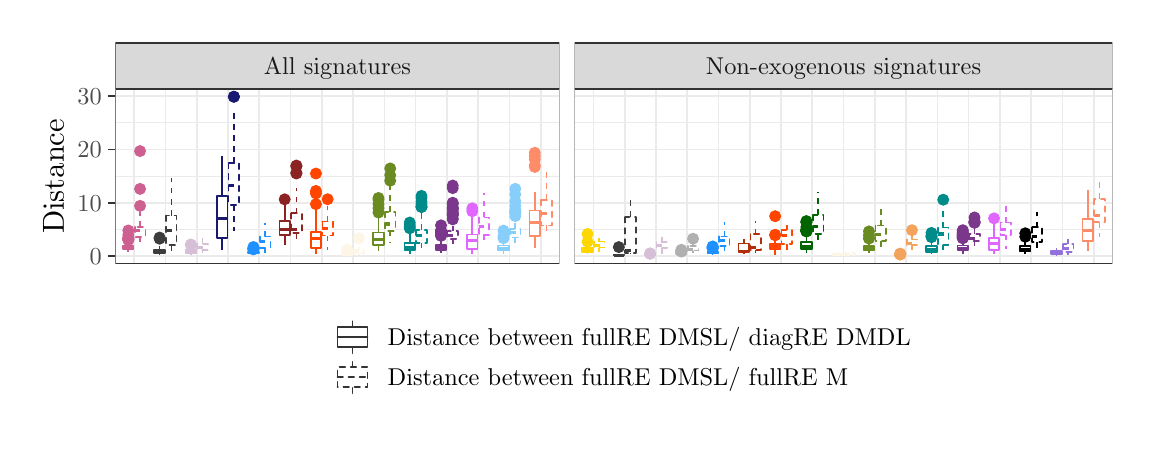
\begin{tikzpicture}[x=1pt,y=1pt]
\definecolor{fillColor}{RGB}{255,255,255}
\path[use as bounding box,fill=fillColor,fill opacity=0.00] (0,0) rectangle (397.48,144.54);
\begin{scope}
\path[clip] (  0.00,  0.00) rectangle (397.48,144.54);
\definecolor{drawColor}{RGB}{255,255,255}
\definecolor{fillColor}{RGB}{255,255,255}

\path[draw=drawColor,line width= 0.6pt,line join=round,line cap=round,fill=fillColor] (  0.00,  0.00) rectangle (397.48,144.54);
\end{scope}
\begin{scope}
\path[clip] ( 31.71, 59.16) rectangle (192.15,122.47);
\definecolor{fillColor}{RGB}{255,255,255}

\path[fill=fillColor] ( 31.71, 59.16) rectangle (192.15,122.47);
\definecolor{drawColor}{gray}{0.92}

\path[draw=drawColor,line width= 0.3pt,line join=round] ( 31.71, 71.67) --
	(192.15, 71.67);

\path[draw=drawColor,line width= 0.3pt,line join=round] ( 31.71, 90.92) --
	(192.15, 90.92);

\path[draw=drawColor,line width= 0.3pt,line join=round] ( 31.71,110.18) --
	(192.15,110.18);

\path[draw=drawColor,line width= 0.6pt,line join=round] ( 31.71, 62.04) --
	(192.15, 62.04);

\path[draw=drawColor,line width= 0.6pt,line join=round] ( 31.71, 81.29) --
	(192.15, 81.29);

\path[draw=drawColor,line width= 0.6pt,line join=round] ( 31.71,100.55) --
	(192.15,100.55);

\path[draw=drawColor,line width= 0.6pt,line join=round] ( 31.71,119.81) --
	(192.15,119.81);

\path[draw=drawColor,line width= 0.6pt,line join=round] ( 38.49, 59.16) --
	( 38.49,122.47);

\path[draw=drawColor,line width= 0.6pt,line join=round] ( 49.79, 59.16) --
	( 49.79,122.47);

\path[draw=drawColor,line width= 0.6pt,line join=round] ( 61.09, 59.16) --
	( 61.09,122.47);

\path[draw=drawColor,line width= 0.6pt,line join=round] ( 72.39, 59.16) --
	( 72.39,122.47);

\path[draw=drawColor,line width= 0.6pt,line join=round] ( 83.69, 59.16) --
	( 83.69,122.47);

\path[draw=drawColor,line width= 0.6pt,line join=round] ( 94.98, 59.16) --
	( 94.98,122.47);

\path[draw=drawColor,line width= 0.6pt,line join=round] (106.28, 59.16) --
	(106.28,122.47);

\path[draw=drawColor,line width= 0.6pt,line join=round] (117.58, 59.16) --
	(117.58,122.47);

\path[draw=drawColor,line width= 0.6pt,line join=round] (128.88, 59.16) --
	(128.88,122.47);

\path[draw=drawColor,line width= 0.6pt,line join=round] (140.18, 59.16) --
	(140.18,122.47);

\path[draw=drawColor,line width= 0.6pt,line join=round] (151.48, 59.16) --
	(151.48,122.47);

\path[draw=drawColor,line width= 0.6pt,line join=round] (162.77, 59.16) --
	(162.77,122.47);

\path[draw=drawColor,line width= 0.6pt,line join=round] (174.07, 59.16) --
	(174.07,122.47);

\path[draw=drawColor,line width= 0.6pt,line join=round] (185.37, 59.16) --
	(185.37,122.47);
\definecolor{drawColor}{RGB}{205,96,144}
\definecolor{fillColor}{RGB}{205,96,144}

\path[draw=drawColor,line width= 0.4pt,line join=round,line cap=round,fill=fillColor] ( 36.37, 69.66) circle (  1.96);

\path[draw=drawColor,line width= 0.4pt,line join=round,line cap=round,fill=fillColor] ( 36.37, 68.58) circle (  1.96);

\path[draw=drawColor,line width= 0.4pt,line join=round,line cap=round,fill=fillColor] ( 36.37, 67.85) circle (  1.96);

\path[draw=drawColor,line width= 0.4pt,line join=round,line cap=round,fill=fillColor] ( 36.37, 68.68) circle (  1.96);

\path[draw=drawColor,line width= 0.4pt,line join=round,line cap=round,fill=fillColor] ( 36.37, 68.01) circle (  1.96);

\path[draw=drawColor,line width= 0.4pt,line join=round,line cap=round,fill=fillColor] ( 36.37, 71.26) circle (  1.96);

\path[draw=drawColor,line width= 0.4pt,line join=round,line cap=round,fill=fillColor] ( 36.37, 67.85) circle (  1.96);

\path[draw=drawColor,line width= 0.4pt,line join=round,line cap=round,fill=fillColor] ( 36.37, 68.35) circle (  1.96);

\path[draw=drawColor,line width= 0.6pt,line join=round] ( 36.37, 65.84) -- ( 36.37, 67.70);

\path[draw=drawColor,line width= 0.6pt,line join=round] ( 36.37, 64.50) -- ( 36.37, 63.40);
\definecolor{fillColor}{RGB}{255,255,255}

\path[draw=drawColor,line width= 0.6pt,line join=round,line cap=round,fill=fillColor] ( 34.47, 65.84) --
	( 34.47, 64.50) --
	( 38.28, 64.50) --
	( 38.28, 65.84) --
	( 34.47, 65.84) --
	cycle;

\path[draw=drawColor,line width= 1.1pt,line join=round] ( 34.47, 65.18) -- ( 38.28, 65.18);
\definecolor{fillColor}{RGB}{205,96,144}

\path[draw=drawColor,line width= 0.4pt,line join=round,line cap=round,fill=fillColor] ( 40.61, 99.95) circle (  1.96);

\path[draw=drawColor,line width= 0.4pt,line join=round,line cap=round,fill=fillColor] ( 40.61, 86.28) circle (  1.96);

\path[draw=drawColor,line width= 0.4pt,line join=round,line cap=round,fill=fillColor] ( 40.61, 80.15) circle (  1.96);

\path[draw=drawColor,line width= 0.6pt,dash pattern=on 2pt off 2pt ,line join=round] ( 40.61, 72.60) -- ( 40.61, 78.10);

\path[draw=drawColor,line width= 0.6pt,dash pattern=on 2pt off 2pt ,line join=round] ( 40.61, 68.93) -- ( 40.61, 64.97);
\definecolor{fillColor}{RGB}{255,255,255}

\path[draw=drawColor,line width= 0.6pt,dash pattern=on 2pt off 2pt ,line join=round,line cap=round,fill=fillColor] ( 38.70, 72.60) --
	( 38.70, 68.93) --
	( 42.52, 68.93) --
	( 42.52, 72.60) --
	( 38.70, 72.60) --
	cycle;

\path[draw=drawColor,line width= 1.1pt,dash pattern=on 2pt off 2pt ,line join=round] ( 38.70, 71.18) -- ( 42.52, 71.18);
\definecolor{drawColor}{gray}{0.24}
\definecolor{fillColor}{gray}{0.24}

\path[draw=drawColor,line width= 0.4pt,line join=round,line cap=round,fill=fillColor] ( 47.67, 68.28) circle (  1.96);

\path[draw=drawColor,line width= 0.4pt,line join=round,line cap=round,fill=fillColor] ( 47.67, 68.70) circle (  1.96);

\path[draw=drawColor,line width= 0.6pt,line join=round] ( 47.67, 64.22) -- ( 47.67, 65.55);

\path[draw=drawColor,line width= 0.6pt,line join=round] ( 47.67, 63.08) -- ( 47.67, 62.49);
\definecolor{fillColor}{RGB}{255,255,255}

\path[draw=drawColor,line width= 0.6pt,line join=round,line cap=round,fill=fillColor] ( 45.76, 64.22) --
	( 45.76, 63.08) --
	( 49.58, 63.08) --
	( 49.58, 64.22) --
	( 45.76, 64.22) --
	cycle;

\path[draw=drawColor,line width= 1.1pt,line join=round] ( 45.76, 63.51) -- ( 49.58, 63.51);

\path[draw=drawColor,line width= 0.6pt,dash pattern=on 2pt off 2pt ,line join=round] ( 51.91, 76.64) -- ( 51.91, 90.10);

\path[draw=drawColor,line width= 0.6pt,dash pattern=on 2pt off 2pt ,line join=round] ( 51.91, 65.90) -- ( 51.91, 63.90);

\path[draw=drawColor,line width= 0.6pt,dash pattern=on 2pt off 2pt ,line join=round,line cap=round,fill=fillColor] ( 50.00, 76.64) --
	( 50.00, 65.90) --
	( 53.81, 65.90) --
	( 53.81, 76.64) --
	( 50.00, 76.64) --
	cycle;

\path[draw=drawColor,line width= 1.1pt,dash pattern=on 2pt off 2pt ,line join=round] ( 50.00, 71.30) -- ( 53.81, 71.30);
\definecolor{drawColor}{RGB}{216,191,216}
\definecolor{fillColor}{RGB}{216,191,216}

\path[draw=drawColor,line width= 0.4pt,line join=round,line cap=round,fill=fillColor] ( 58.97, 65.99) circle (  1.96);

\path[draw=drawColor,line width= 0.4pt,line join=round,line cap=round,fill=fillColor] ( 58.97, 66.21) circle (  1.96);

\path[draw=drawColor,line width= 0.6pt,line join=round] ( 58.97, 64.12) -- ( 58.97, 65.41);

\path[draw=drawColor,line width= 0.6pt,line join=round] ( 58.97, 62.95) -- ( 58.97, 62.32);
\definecolor{fillColor}{RGB}{255,255,255}

\path[draw=drawColor,line width= 0.6pt,line join=round,line cap=round,fill=fillColor] ( 57.06, 64.12) --
	( 57.06, 62.95) --
	( 60.88, 62.95) --
	( 60.88, 64.12) --
	( 57.06, 64.12) --
	cycle;

\path[draw=drawColor,line width= 1.1pt,line join=round] ( 57.06, 63.45) -- ( 60.88, 63.45);

\path[draw=drawColor,line width= 0.6pt,dash pattern=on 2pt off 2pt ,line join=round] ( 63.21, 66.45) -- ( 63.21, 69.22);

\path[draw=drawColor,line width= 0.6pt,dash pattern=on 2pt off 2pt ,line join=round] ( 63.21, 64.23) -- ( 63.21, 63.00);

\path[draw=drawColor,line width= 0.6pt,dash pattern=on 2pt off 2pt ,line join=round,line cap=round,fill=fillColor] ( 61.30, 66.45) --
	( 61.30, 64.23) --
	( 65.11, 64.23) --
	( 65.11, 66.45) --
	( 61.30, 66.45) --
	cycle;

\path[draw=drawColor,line width= 1.1pt,dash pattern=on 2pt off 2pt ,line join=round] ( 61.30, 65.04) -- ( 65.11, 65.04);
\definecolor{drawColor}{RGB}{25,25,112}

\path[draw=drawColor,line width= 0.6pt,line join=round] ( 70.27, 83.64) -- ( 70.27, 98.11);

\path[draw=drawColor,line width= 0.6pt,line join=round] ( 70.27, 68.51) -- ( 70.27, 64.38);

\path[draw=drawColor,line width= 0.6pt,line join=round,line cap=round,fill=fillColor] ( 68.36, 83.64) --
	( 68.36, 68.51) --
	( 72.17, 68.51) --
	( 72.17, 83.64) --
	( 68.36, 83.64) --
	cycle;

\path[draw=drawColor,line width= 1.1pt,line join=round] ( 68.36, 75.65) -- ( 72.17, 75.65);
\definecolor{fillColor}{RGB}{25,25,112}

\path[draw=drawColor,line width= 0.4pt,line join=round,line cap=round,fill=fillColor] ( 74.51,119.59) circle (  1.96);

\path[draw=drawColor,line width= 0.4pt,line join=round,line cap=round,fill=fillColor] ( 74.51,119.59) circle (  1.96);

\path[draw=drawColor,line width= 0.6pt,dash pattern=on 2pt off 2pt ,line join=round] ( 74.51, 95.70) -- ( 74.51,115.36);

\path[draw=drawColor,line width= 0.6pt,dash pattern=on 2pt off 2pt ,line join=round] ( 74.51, 80.47) -- ( 74.51, 71.08);
\definecolor{fillColor}{RGB}{255,255,255}

\path[draw=drawColor,line width= 0.6pt,dash pattern=on 2pt off 2pt ,line join=round,line cap=round,fill=fillColor] ( 72.60, 95.70) --
	( 72.60, 80.47) --
	( 76.41, 80.47) --
	( 76.41, 95.70) --
	( 72.60, 95.70) --
	cycle;

\path[draw=drawColor,line width= 1.1pt,dash pattern=on 2pt off 2pt ,line join=round] ( 72.60, 87.43) -- ( 76.41, 87.43);
\definecolor{drawColor}{RGB}{30,144,255}
\definecolor{fillColor}{RGB}{30,144,255}

\path[draw=drawColor,line width= 0.4pt,line join=round,line cap=round,fill=fillColor] ( 81.57, 64.49) circle (  1.96);

\path[draw=drawColor,line width= 0.4pt,line join=round,line cap=round,fill=fillColor] ( 81.57, 64.45) circle (  1.96);

\path[draw=drawColor,line width= 0.4pt,line join=round,line cap=round,fill=fillColor] ( 81.57, 64.64) circle (  1.96);

\path[draw=drawColor,line width= 0.4pt,line join=round,line cap=round,fill=fillColor] ( 81.57, 65.28) circle (  1.96);

\path[draw=drawColor,line width= 0.4pt,line join=round,line cap=round,fill=fillColor] ( 81.57, 64.78) circle (  1.96);

\path[draw=drawColor,line width= 0.6pt,line join=round] ( 81.57, 63.58) -- ( 81.57, 64.34);

\path[draw=drawColor,line width= 0.6pt,line join=round] ( 81.57, 63.04) -- ( 81.57, 62.50);
\definecolor{fillColor}{RGB}{255,255,255}

\path[draw=drawColor,line width= 0.6pt,line join=round,line cap=round,fill=fillColor] ( 79.66, 63.58) --
	( 79.66, 63.04) --
	( 83.47, 63.04) --
	( 83.47, 63.58) --
	( 79.66, 63.58) --
	cycle;

\path[draw=drawColor,line width= 1.1pt,line join=round] ( 79.66, 63.33) -- ( 83.47, 63.33);

\path[draw=drawColor,line width= 0.6pt,dash pattern=on 2pt off 2pt ,line join=round] ( 85.80, 69.09) -- ( 85.80, 74.06);

\path[draw=drawColor,line width= 0.6pt,dash pattern=on 2pt off 2pt ,line join=round] ( 85.80, 65.02) -- ( 85.80, 63.28);

\path[draw=drawColor,line width= 0.6pt,dash pattern=on 2pt off 2pt ,line join=round,line cap=round,fill=fillColor] ( 83.90, 69.09) --
	( 83.90, 65.02) --
	( 87.71, 65.02) --
	( 87.71, 69.09) --
	( 83.90, 69.09) --
	cycle;

\path[draw=drawColor,line width= 1.1pt,dash pattern=on 2pt off 2pt ,line join=round] ( 83.90, 67.36) -- ( 87.71, 67.36);
\definecolor{drawColor}{RGB}{139,35,35}
\definecolor{fillColor}{RGB}{139,35,35}

\path[draw=drawColor,line width= 0.4pt,line join=round,line cap=round,fill=fillColor] ( 92.87, 82.51) circle (  1.96);

\path[draw=drawColor,line width= 0.6pt,line join=round] ( 92.87, 74.57) -- ( 92.87, 81.22);

\path[draw=drawColor,line width= 0.6pt,line join=round] ( 92.87, 69.60) -- ( 92.87, 65.98);
\definecolor{fillColor}{RGB}{255,255,255}

\path[draw=drawColor,line width= 0.6pt,line join=round,line cap=round,fill=fillColor] ( 90.96, 74.57) --
	( 90.96, 69.60) --
	( 94.77, 69.60) --
	( 94.77, 74.57) --
	( 90.96, 74.57) --
	cycle;

\path[draw=drawColor,line width= 1.1pt,line join=round] ( 90.96, 71.46) -- ( 94.77, 71.46);
\definecolor{fillColor}{RGB}{139,35,35}

\path[draw=drawColor,line width= 0.4pt,line join=round,line cap=round,fill=fillColor] ( 97.10, 94.40) circle (  1.96);

\path[draw=drawColor,line width= 0.4pt,line join=round,line cap=round,fill=fillColor] ( 97.10, 91.84) circle (  1.96);

\path[draw=drawColor,line width= 0.4pt,line join=round,line cap=round,fill=fillColor] ( 97.10, 94.72) circle (  1.96);

\path[draw=drawColor,line width= 0.4pt,line join=round,line cap=round,fill=fillColor] ( 97.10, 92.13) circle (  1.96);

\path[draw=drawColor,line width= 0.6pt,dash pattern=on 2pt off 2pt ,line join=round] ( 97.10, 77.49) -- ( 97.10, 86.48);

\path[draw=drawColor,line width= 0.6pt,dash pattern=on 2pt off 2pt ,line join=round] ( 97.10, 70.26) -- ( 97.10, 67.41);
\definecolor{fillColor}{RGB}{255,255,255}

\path[draw=drawColor,line width= 0.6pt,dash pattern=on 2pt off 2pt ,line join=round,line cap=round,fill=fillColor] ( 95.20, 77.49) --
	( 95.20, 70.26) --
	( 99.01, 70.26) --
	( 99.01, 77.49) --
	( 95.20, 77.49) --
	cycle;

\path[draw=drawColor,line width= 1.1pt,dash pattern=on 2pt off 2pt ,line join=round] ( 95.20, 71.75) -- ( 99.01, 71.75);
\definecolor{drawColor}{RGB}{255,69,0}
\definecolor{fillColor}{RGB}{255,69,0}

\path[draw=drawColor,line width= 0.4pt,line join=round,line cap=round,fill=fillColor] (104.16, 84.63) circle (  1.96);

\path[draw=drawColor,line width= 0.4pt,line join=round,line cap=round,fill=fillColor] (104.16, 91.83) circle (  1.96);

\path[draw=drawColor,line width= 0.4pt,line join=round,line cap=round,fill=fillColor] (104.16, 85.54) circle (  1.96);

\path[draw=drawColor,line width= 0.4pt,line join=round,line cap=round,fill=fillColor] (104.16, 80.77) circle (  1.96);

\path[draw=drawColor,line width= 0.6pt,line join=round] (104.16, 70.59) -- (104.16, 78.95);

\path[draw=drawColor,line width= 0.6pt,line join=round] (104.16, 64.93) -- (104.16, 62.69);
\definecolor{fillColor}{RGB}{255,255,255}

\path[draw=drawColor,line width= 0.6pt,line join=round,line cap=round,fill=fillColor] (102.26, 70.59) --
	(102.26, 64.93) --
	(106.07, 64.93) --
	(106.07, 70.59) --
	(102.26, 70.59) --
	cycle;

\path[draw=drawColor,line width= 1.1pt,line join=round] (102.26, 68.46) -- (106.07, 68.46);
\definecolor{fillColor}{RGB}{255,69,0}

\path[draw=drawColor,line width= 0.4pt,line join=round,line cap=round,fill=fillColor] (108.40, 82.55) circle (  1.96);

\path[draw=drawColor,line width= 0.6pt,dash pattern=on 2pt off 2pt ,line join=round] (108.40, 74.49) -- (108.40, 80.04);

\path[draw=drawColor,line width= 0.6pt,dash pattern=on 2pt off 2pt ,line join=round] (108.40, 69.38) -- (108.40, 64.09);
\definecolor{fillColor}{RGB}{255,255,255}

\path[draw=drawColor,line width= 0.6pt,dash pattern=on 2pt off 2pt ,line join=round,line cap=round,fill=fillColor] (106.49, 74.49) --
	(106.49, 69.38) --
	(110.31, 69.38) --
	(110.31, 74.49) --
	(106.49, 74.49) --
	cycle;

\path[draw=drawColor,line width= 1.1pt,dash pattern=on 2pt off 2pt ,line join=round] (106.49, 72.02) -- (110.31, 72.02);
\definecolor{drawColor}{RGB}{253,245,230}
\definecolor{fillColor}{RGB}{253,245,230}

\path[draw=drawColor,line width= 0.4pt,line join=round,line cap=round,fill=fillColor] (115.46, 64.26) circle (  1.96);

\path[draw=drawColor,line width= 0.4pt,line join=round,line cap=round,fill=fillColor] (115.46, 63.97) circle (  1.96);

\path[draw=drawColor,line width= 0.6pt,line join=round] (115.46, 63.06) -- (115.46, 63.85);

\path[draw=drawColor,line width= 0.6pt,line join=round] (115.46, 62.47) -- (115.46, 62.22);
\definecolor{fillColor}{RGB}{255,255,255}

\path[draw=drawColor,line width= 0.6pt,line join=round,line cap=round,fill=fillColor] (113.56, 63.06) --
	(113.56, 62.47) --
	(117.37, 62.47) --
	(117.37, 63.06) --
	(113.56, 63.06) --
	cycle;

\path[draw=drawColor,line width= 1.1pt,line join=round] (113.56, 62.79) -- (117.37, 62.79);
\definecolor{fillColor}{RGB}{253,245,230}

\path[draw=drawColor,line width= 0.4pt,line join=round,line cap=round,fill=fillColor] (119.70, 68.42) circle (  1.96);

\path[draw=drawColor,line width= 0.6pt,dash pattern=on 2pt off 2pt ,line join=round] (119.70, 64.14) -- (119.70, 65.38);

\path[draw=drawColor,line width= 0.6pt,dash pattern=on 2pt off 2pt ,line join=round] (119.70, 63.10) -- (119.70, 62.56);
\definecolor{fillColor}{RGB}{255,255,255}

\path[draw=drawColor,line width= 0.6pt,dash pattern=on 2pt off 2pt ,line join=round,line cap=round,fill=fillColor] (117.79, 64.14) --
	(117.79, 63.10) --
	(121.61, 63.10) --
	(121.61, 64.14) --
	(117.79, 64.14) --
	cycle;

\path[draw=drawColor,line width= 1.1pt,dash pattern=on 2pt off 2pt ,line join=round] (117.79, 63.63) -- (121.61, 63.63);
\definecolor{drawColor}{RGB}{105,139,34}
\definecolor{fillColor}{RGB}{105,139,34}

\path[draw=drawColor,line width= 0.4pt,line join=round,line cap=round,fill=fillColor] (126.76, 83.00) circle (  1.96);

\path[draw=drawColor,line width= 0.4pt,line join=round,line cap=round,fill=fillColor] (126.76, 80.83) circle (  1.96);

\path[draw=drawColor,line width= 0.4pt,line join=round,line cap=round,fill=fillColor] (126.76, 79.29) circle (  1.96);

\path[draw=drawColor,line width= 0.4pt,line join=round,line cap=round,fill=fillColor] (126.76, 77.74) circle (  1.96);

\path[draw=drawColor,line width= 0.4pt,line join=round,line cap=round,fill=fillColor] (126.76, 82.43) circle (  1.96);

\path[draw=drawColor,line width= 0.6pt,line join=round] (126.76, 70.55) -- (126.76, 75.59);

\path[draw=drawColor,line width= 0.6pt,line join=round] (126.76, 66.00) -- (126.76, 63.86);
\definecolor{fillColor}{RGB}{255,255,255}

\path[draw=drawColor,line width= 0.6pt,line join=round,line cap=round,fill=fillColor] (124.85, 70.55) --
	(124.85, 66.00) --
	(128.67, 66.00) --
	(128.67, 70.55) --
	(124.85, 70.55) --
	cycle;

\path[draw=drawColor,line width= 1.1pt,line join=round] (124.85, 68.04) -- (128.67, 68.04);
\definecolor{fillColor}{RGB}{105,139,34}

\path[draw=drawColor,line width= 0.4pt,line join=round,line cap=round,fill=fillColor] (131.00, 93.68) circle (  1.96);

\path[draw=drawColor,line width= 0.4pt,line join=round,line cap=round,fill=fillColor] (131.00, 89.24) circle (  1.96);

\path[draw=drawColor,line width= 0.4pt,line join=round,line cap=round,fill=fillColor] (131.00, 91.22) circle (  1.96);

\path[draw=drawColor,line width= 0.6pt,dash pattern=on 2pt off 2pt ,line join=round] (131.00, 77.99) -- (131.00, 87.87);

\path[draw=drawColor,line width= 0.6pt,dash pattern=on 2pt off 2pt ,line join=round] (131.00, 71.16) -- (131.00, 67.03);
\definecolor{fillColor}{RGB}{255,255,255}

\path[draw=drawColor,line width= 0.6pt,dash pattern=on 2pt off 2pt ,line join=round,line cap=round,fill=fillColor] (129.09, 77.99) --
	(129.09, 71.16) --
	(132.90, 71.16) --
	(132.90, 77.99) --
	(129.09, 77.99) --
	cycle;

\path[draw=drawColor,line width= 1.1pt,dash pattern=on 2pt off 2pt ,line join=round] (129.09, 73.59) -- (132.90, 73.59);
\definecolor{drawColor}{RGB}{0,139,139}
\definecolor{fillColor}{RGB}{0,139,139}

\path[draw=drawColor,line width= 0.4pt,line join=round,line cap=round,fill=fillColor] (138.06, 72.51) circle (  1.96);

\path[draw=drawColor,line width= 0.4pt,line join=round,line cap=round,fill=fillColor] (138.06, 74.13) circle (  1.96);

\path[draw=drawColor,line width= 0.4pt,line join=round,line cap=round,fill=fillColor] (138.06, 73.25) circle (  1.96);

\path[draw=drawColor,line width= 0.4pt,line join=round,line cap=round,fill=fillColor] (138.06, 72.04) circle (  1.96);

\path[draw=drawColor,line width= 0.6pt,line join=round] (138.06, 66.68) -- (138.06, 70.46);

\path[draw=drawColor,line width= 0.6pt,line join=round] (138.06, 64.09) -- (138.06, 62.75);
\definecolor{fillColor}{RGB}{255,255,255}

\path[draw=drawColor,line width= 0.6pt,line join=round,line cap=round,fill=fillColor] (136.15, 66.68) --
	(136.15, 64.09) --
	(139.97, 64.09) --
	(139.97, 66.68) --
	(136.15, 66.68) --
	cycle;

\path[draw=drawColor,line width= 1.1pt,line join=round] (136.15, 65.01) -- (139.97, 65.01);
\definecolor{fillColor}{RGB}{0,139,139}

\path[draw=drawColor,line width= 0.4pt,line join=round,line cap=round,fill=fillColor] (142.30, 79.82) circle (  1.96);

\path[draw=drawColor,line width= 0.4pt,line join=round,line cap=round,fill=fillColor] (142.30, 83.76) circle (  1.96);

\path[draw=drawColor,line width= 0.4pt,line join=round,line cap=round,fill=fillColor] (142.30, 82.99) circle (  1.96);

\path[draw=drawColor,line width= 0.4pt,line join=round,line cap=round,fill=fillColor] (142.30, 81.64) circle (  1.96);

\path[draw=drawColor,line width= 0.4pt,line join=round,line cap=round,fill=fillColor] (142.30, 79.74) circle (  1.96);

\path[draw=drawColor,line width= 0.4pt,line join=round,line cap=round,fill=fillColor] (142.30, 79.80) circle (  1.96);

\path[draw=drawColor,line width= 0.4pt,line join=round,line cap=round,fill=fillColor] (142.30, 80.68) circle (  1.96);

\path[draw=drawColor,line width= 0.6pt,dash pattern=on 2pt off 2pt ,line join=round] (142.30, 71.54) -- (142.30, 77.68);

\path[draw=drawColor,line width= 0.6pt,dash pattern=on 2pt off 2pt ,line join=round] (142.30, 66.79) -- (142.30, 63.63);
\definecolor{fillColor}{RGB}{255,255,255}

\path[draw=drawColor,line width= 0.6pt,dash pattern=on 2pt off 2pt ,line join=round,line cap=round,fill=fillColor] (140.39, 71.54) --
	(140.39, 66.79) --
	(144.20, 66.79) --
	(144.20, 71.54) --
	(140.39, 71.54) --
	cycle;

\path[draw=drawColor,line width= 1.1pt,dash pattern=on 2pt off 2pt ,line join=round] (140.39, 69.56) -- (144.20, 69.56);
\definecolor{drawColor}{RGB}{122,55,139}
\definecolor{fillColor}{RGB}{122,55,139}

\path[draw=drawColor,line width= 0.4pt,line join=round,line cap=round,fill=fillColor] (149.36, 71.33) circle (  1.96);

\path[draw=drawColor,line width= 0.4pt,line join=round,line cap=round,fill=fillColor] (149.36, 70.36) circle (  1.96);

\path[draw=drawColor,line width= 0.4pt,line join=round,line cap=round,fill=fillColor] (149.36, 69.32) circle (  1.96);

\path[draw=drawColor,line width= 0.4pt,line join=round,line cap=round,fill=fillColor] (149.36, 70.09) circle (  1.96);

\path[draw=drawColor,line width= 0.4pt,line join=round,line cap=round,fill=fillColor] (149.36, 69.57) circle (  1.96);

\path[draw=drawColor,line width= 0.4pt,line join=round,line cap=round,fill=fillColor] (149.36, 70.76) circle (  1.96);

\path[draw=drawColor,line width= 0.4pt,line join=round,line cap=round,fill=fillColor] (149.36, 73.11) circle (  1.96);

\path[draw=drawColor,line width= 0.6pt,line join=round] (149.36, 66.12) -- (149.36, 68.86);

\path[draw=drawColor,line width= 0.6pt,line join=round] (149.36, 64.19) -- (149.36, 63.18);
\definecolor{fillColor}{RGB}{255,255,255}

\path[draw=drawColor,line width= 0.6pt,line join=round,line cap=round,fill=fillColor] (147.45, 66.12) --
	(147.45, 64.19) --
	(151.26, 64.19) --
	(151.26, 66.12) --
	(147.45, 66.12) --
	cycle;

\path[draw=drawColor,line width= 1.1pt,line join=round] (147.45, 65.04) -- (151.26, 65.04);
\definecolor{fillColor}{RGB}{122,55,139}

\path[draw=drawColor,line width= 0.4pt,line join=round,line cap=round,fill=fillColor] (153.59, 87.50) circle (  1.96);

\path[draw=drawColor,line width= 0.4pt,line join=round,line cap=round,fill=fillColor] (153.59, 77.07) circle (  1.96);

\path[draw=drawColor,line width= 0.4pt,line join=round,line cap=round,fill=fillColor] (153.59, 78.05) circle (  1.96);

\path[draw=drawColor,line width= 0.4pt,line join=round,line cap=round,fill=fillColor] (153.59, 81.28) circle (  1.96);

\path[draw=drawColor,line width= 0.4pt,line join=round,line cap=round,fill=fillColor] (153.59, 80.87) circle (  1.96);

\path[draw=drawColor,line width= 0.4pt,line join=round,line cap=round,fill=fillColor] (153.59, 78.91) circle (  1.96);

\path[draw=drawColor,line width= 0.4pt,line join=round,line cap=round,fill=fillColor] (153.59, 86.56) circle (  1.96);

\path[draw=drawColor,line width= 0.4pt,line join=round,line cap=round,fill=fillColor] (153.59, 77.65) circle (  1.96);

\path[draw=drawColor,line width= 0.4pt,line join=round,line cap=round,fill=fillColor] (153.59, 79.70) circle (  1.96);

\path[draw=drawColor,line width= 0.4pt,line join=round,line cap=round,fill=fillColor] (153.59, 81.01) circle (  1.96);

\path[draw=drawColor,line width= 0.4pt,line join=round,line cap=round,fill=fillColor] (153.59, 76.80) circle (  1.96);

\path[draw=drawColor,line width= 0.4pt,line join=round,line cap=round,fill=fillColor] (153.59, 76.81) circle (  1.96);

\path[draw=drawColor,line width= 0.4pt,line join=round,line cap=round,fill=fillColor] (153.59, 79.02) circle (  1.96);

\path[draw=drawColor,line width= 0.4pt,line join=round,line cap=round,fill=fillColor] (153.59, 79.41) circle (  1.96);

\path[draw=drawColor,line width= 0.4pt,line join=round,line cap=round,fill=fillColor] (153.59, 75.26) circle (  1.96);

\path[draw=drawColor,line width= 0.4pt,line join=round,line cap=round,fill=fillColor] (153.59, 75.55) circle (  1.96);

\path[draw=drawColor,line width= 0.4pt,line join=round,line cap=round,fill=fillColor] (153.59, 77.16) circle (  1.96);

\path[draw=drawColor,line width= 0.6pt,dash pattern=on 2pt off 2pt ,line join=round] (153.59, 70.98) -- (153.59, 74.06);

\path[draw=drawColor,line width= 0.6pt,dash pattern=on 2pt off 2pt ,line join=round] (153.59, 68.17) -- (153.59, 66.22);
\definecolor{fillColor}{RGB}{255,255,255}

\path[draw=drawColor,line width= 0.6pt,dash pattern=on 2pt off 2pt ,line join=round,line cap=round,fill=fillColor] (151.69, 70.98) --
	(151.69, 68.17) --
	(155.50, 68.17) --
	(155.50, 70.98) --
	(151.69, 70.98) --
	cycle;

\path[draw=drawColor,line width= 1.1pt,dash pattern=on 2pt off 2pt ,line join=round] (151.69, 69.56) -- (155.50, 69.56);
\definecolor{drawColor}{RGB}{224,102,255}
\definecolor{fillColor}{RGB}{224,102,255}

\path[draw=drawColor,line width= 0.4pt,line join=round,line cap=round,fill=fillColor] (160.66, 78.21) circle (  1.96);

\path[draw=drawColor,line width= 0.4pt,line join=round,line cap=round,fill=fillColor] (160.66, 79.25) circle (  1.96);

\path[draw=drawColor,line width= 0.6pt,line join=round] (160.66, 69.78) -- (160.66, 76.14);

\path[draw=drawColor,line width= 0.6pt,line join=round] (160.66, 64.49) -- (160.66, 62.91);
\definecolor{fillColor}{RGB}{255,255,255}

\path[draw=drawColor,line width= 0.6pt,line join=round,line cap=round,fill=fillColor] (158.75, 69.78) --
	(158.75, 64.49) --
	(162.56, 64.49) --
	(162.56, 69.78) --
	(158.75, 69.78) --
	cycle;

\path[draw=drawColor,line width= 1.1pt,line join=round] (158.75, 67.80) -- (162.56, 67.80);

\path[draw=drawColor,line width= 0.6pt,dash pattern=on 2pt off 2pt ,line join=round] (164.89, 75.96) -- (164.89, 84.66);

\path[draw=drawColor,line width= 0.6pt,dash pattern=on 2pt off 2pt ,line join=round] (164.89, 69.71) -- (164.89, 65.77);

\path[draw=drawColor,line width= 0.6pt,dash pattern=on 2pt off 2pt ,line join=round,line cap=round,fill=fillColor] (162.99, 75.96) --
	(162.99, 69.71) --
	(166.80, 69.71) --
	(166.80, 75.96) --
	(162.99, 75.96) --
	cycle;

\path[draw=drawColor,line width= 1.1pt,dash pattern=on 2pt off 2pt ,line join=round] (162.99, 72.53) -- (166.80, 72.53);
\definecolor{drawColor}{RGB}{135,206,250}
\definecolor{fillColor}{RGB}{135,206,250}

\path[draw=drawColor,line width= 0.4pt,line join=round,line cap=round,fill=fillColor] (171.95, 68.73) circle (  1.96);

\path[draw=drawColor,line width= 0.4pt,line join=round,line cap=round,fill=fillColor] (171.95, 71.21) circle (  1.96);

\path[draw=drawColor,line width= 0.4pt,line join=round,line cap=round,fill=fillColor] (171.95, 69.46) circle (  1.96);

\path[draw=drawColor,line width= 0.4pt,line join=round,line cap=round,fill=fillColor] (171.95, 68.47) circle (  1.96);

\path[draw=drawColor,line width= 0.6pt,line join=round] (171.95, 65.78) -- (171.95, 68.43);

\path[draw=drawColor,line width= 0.6pt,line join=round] (171.95, 64.00) -- (171.95, 62.90);
\definecolor{fillColor}{RGB}{255,255,255}

\path[draw=drawColor,line width= 0.6pt,line join=round,line cap=round,fill=fillColor] (170.05, 65.78) --
	(170.05, 64.00) --
	(173.86, 64.00) --
	(173.86, 65.78) --
	(170.05, 65.78) --
	cycle;

\path[draw=drawColor,line width= 1.1pt,line join=round] (170.05, 64.60) -- (173.86, 64.60);
\definecolor{fillColor}{RGB}{135,206,250}

\path[draw=drawColor,line width= 0.4pt,line join=round,line cap=round,fill=fillColor] (176.19, 81.80) circle (  1.96);

\path[draw=drawColor,line width= 0.4pt,line join=round,line cap=round,fill=fillColor] (176.19, 84.28) circle (  1.96);

\path[draw=drawColor,line width= 0.4pt,line join=round,line cap=round,fill=fillColor] (176.19, 76.46) circle (  1.96);

\path[draw=drawColor,line width= 0.4pt,line join=round,line cap=round,fill=fillColor] (176.19, 78.68) circle (  1.96);

\path[draw=drawColor,line width= 0.4pt,line join=round,line cap=round,fill=fillColor] (176.19, 80.16) circle (  1.96);

\path[draw=drawColor,line width= 0.4pt,line join=round,line cap=round,fill=fillColor] (176.19, 86.29) circle (  1.96);

\path[draw=drawColor,line width= 0.4pt,line join=round,line cap=round,fill=fillColor] (176.19, 77.85) circle (  1.96);

\path[draw=drawColor,line width= 0.4pt,line join=round,line cap=round,fill=fillColor] (176.19, 78.02) circle (  1.96);

\path[draw=drawColor,line width= 0.4pt,line join=round,line cap=round,fill=fillColor] (176.19, 77.52) circle (  1.96);

\path[draw=drawColor,line width= 0.6pt,dash pattern=on 2pt off 2pt ,line join=round] (176.19, 71.82) -- (176.19, 76.04);

\path[draw=drawColor,line width= 0.6pt,dash pattern=on 2pt off 2pt ,line join=round] (176.19, 68.77) -- (176.19, 65.99);
\definecolor{fillColor}{RGB}{255,255,255}

\path[draw=drawColor,line width= 0.6pt,dash pattern=on 2pt off 2pt ,line join=round,line cap=round,fill=fillColor] (174.29, 71.82) --
	(174.29, 68.77) --
	(178.10, 68.77) --
	(178.10, 71.82) --
	(174.29, 71.82) --
	cycle;

\path[draw=drawColor,line width= 1.1pt,dash pattern=on 2pt off 2pt ,line join=round] (174.29, 70.36) -- (178.10, 70.36);
\definecolor{drawColor}{RGB}{255,140,105}
\definecolor{fillColor}{RGB}{255,140,105}

\path[draw=drawColor,line width= 0.4pt,line join=round,line cap=round,fill=fillColor] (183.25, 94.22) circle (  1.96);

\path[draw=drawColor,line width= 0.4pt,line join=round,line cap=round,fill=fillColor] (183.25, 96.95) circle (  1.96);

\path[draw=drawColor,line width= 0.4pt,line join=round,line cap=round,fill=fillColor] (183.25, 98.09) circle (  1.96);

\path[draw=drawColor,line width= 0.4pt,line join=round,line cap=round,fill=fillColor] (183.25, 94.84) circle (  1.96);

\path[draw=drawColor,line width= 0.4pt,line join=round,line cap=round,fill=fillColor] (183.25, 99.33) circle (  1.96);

\path[draw=drawColor,line width= 0.6pt,line join=round] (183.25, 78.43) -- (183.25, 84.98);

\path[draw=drawColor,line width= 0.6pt,line join=round] (183.25, 69.19) -- (183.25, 64.89);
\definecolor{fillColor}{RGB}{255,255,255}

\path[draw=drawColor,line width= 0.6pt,line join=round,line cap=round,fill=fillColor] (181.35, 78.43) --
	(181.35, 69.19) --
	(185.16, 69.19) --
	(185.16, 78.43) --
	(181.35, 78.43) --
	cycle;

\path[draw=drawColor,line width= 1.1pt,line join=round] (181.35, 74.19) -- (185.16, 74.19);

\path[draw=drawColor,line width= 0.6pt,dash pattern=on 2pt off 2pt ,line join=round] (187.49, 82.32) -- (187.49, 93.06);

\path[draw=drawColor,line width= 0.6pt,dash pattern=on 2pt off 2pt ,line join=round] (187.49, 73.10) -- (187.49, 69.73);

\path[draw=drawColor,line width= 0.6pt,dash pattern=on 2pt off 2pt ,line join=round,line cap=round,fill=fillColor] (185.58, 82.32) --
	(185.58, 73.10) --
	(189.40, 73.10) --
	(189.40, 82.32) --
	(185.58, 82.32) --
	cycle;

\path[draw=drawColor,line width= 1.1pt,dash pattern=on 2pt off 2pt ,line join=round] (185.58, 77.25) -- (189.40, 77.25);
\definecolor{drawColor}{gray}{0.20}

\path[draw=drawColor,line width= 0.6pt,line join=round,line cap=round] ( 31.71, 59.16) rectangle (192.15,122.47);
\end{scope}
\begin{scope}
\path[clip] (197.65, 59.16) rectangle (391.98,122.47);
\definecolor{fillColor}{RGB}{255,255,255}

\path[fill=fillColor] (197.65, 59.16) rectangle (391.98,122.47);
\definecolor{drawColor}{gray}{0.92}

\path[draw=drawColor,line width= 0.3pt,line join=round] (197.65, 71.67) --
	(391.98, 71.67);

\path[draw=drawColor,line width= 0.3pt,line join=round] (197.65, 90.92) --
	(391.98, 90.92);

\path[draw=drawColor,line width= 0.3pt,line join=round] (197.65,110.18) --
	(391.98,110.18);

\path[draw=drawColor,line width= 0.6pt,line join=round] (197.65, 62.04) --
	(391.98, 62.04);

\path[draw=drawColor,line width= 0.6pt,line join=round] (197.65, 81.29) --
	(391.98, 81.29);

\path[draw=drawColor,line width= 0.6pt,line join=round] (197.65,100.55) --
	(391.98,100.55);

\path[draw=drawColor,line width= 0.6pt,line join=round] (197.65,119.81) --
	(391.98,119.81);

\path[draw=drawColor,line width= 0.6pt,line join=round] (204.43, 59.16) --
	(204.43,122.47);

\path[draw=drawColor,line width= 0.6pt,line join=round] (215.73, 59.16) --
	(215.73,122.47);

\path[draw=drawColor,line width= 0.6pt,line join=round] (227.03, 59.16) --
	(227.03,122.47);

\path[draw=drawColor,line width= 0.6pt,line join=round] (238.33, 59.16) --
	(238.33,122.47);

\path[draw=drawColor,line width= 0.6pt,line join=round] (249.62, 59.16) --
	(249.62,122.47);

\path[draw=drawColor,line width= 0.6pt,line join=round] (260.92, 59.16) --
	(260.92,122.47);

\path[draw=drawColor,line width= 0.6pt,line join=round] (272.22, 59.16) --
	(272.22,122.47);

\path[draw=drawColor,line width= 0.6pt,line join=round] (283.52, 59.16) --
	(283.52,122.47);

\path[draw=drawColor,line width= 0.6pt,line join=round] (294.82, 59.16) --
	(294.82,122.47);

\path[draw=drawColor,line width= 0.6pt,line join=round] (306.12, 59.16) --
	(306.12,122.47);

\path[draw=drawColor,line width= 0.6pt,line join=round] (317.41, 59.16) --
	(317.41,122.47);

\path[draw=drawColor,line width= 0.6pt,line join=round] (328.71, 59.16) --
	(328.71,122.47);

\path[draw=drawColor,line width= 0.6pt,line join=round] (340.01, 59.16) --
	(340.01,122.47);

\path[draw=drawColor,line width= 0.6pt,line join=round] (351.31, 59.16) --
	(351.31,122.47);

\path[draw=drawColor,line width= 0.6pt,line join=round] (362.61, 59.16) --
	(362.61,122.47);

\path[draw=drawColor,line width= 0.6pt,line join=round] (373.91, 59.16) --
	(373.91,122.47);

\path[draw=drawColor,line width= 0.6pt,line join=round] (385.21, 59.16) --
	(385.21,122.47);
\definecolor{drawColor}{RGB}{255,215,0}
\definecolor{fillColor}{RGB}{255,215,0}

\path[draw=drawColor,line width= 0.4pt,line join=round,line cap=round,fill=fillColor] (202.31, 67.20) circle (  1.96);

\path[draw=drawColor,line width= 0.4pt,line join=round,line cap=round,fill=fillColor] (202.31, 70.00) circle (  1.96);

\path[draw=drawColor,line width= 0.6pt,line join=round] (202.31, 64.82) -- (202.31, 66.33);

\path[draw=drawColor,line width= 0.6pt,line join=round] (202.31, 63.55) -- (202.31, 62.67);
\definecolor{fillColor}{RGB}{255,255,255}

\path[draw=drawColor,line width= 0.6pt,line join=round,line cap=round,fill=fillColor] (200.40, 64.82) --
	(200.40, 63.55) --
	(204.22, 63.55) --
	(204.22, 64.82) --
	(200.40, 64.82) --
	cycle;

\path[draw=drawColor,line width= 1.1pt,line join=round] (200.40, 63.89) -- (204.22, 63.89);

\path[draw=drawColor,line width= 0.6pt,dash pattern=on 2pt off 2pt ,line join=round] (206.55, 67.26) -- (206.55, 68.66);

\path[draw=drawColor,line width= 0.6pt,dash pattern=on 2pt off 2pt ,line join=round] (206.55, 65.08) -- (206.55, 63.55);

\path[draw=drawColor,line width= 0.6pt,dash pattern=on 2pt off 2pt ,line join=round,line cap=round,fill=fillColor] (204.64, 67.26) --
	(204.64, 65.08) --
	(208.46, 65.08) --
	(208.46, 67.26) --
	(204.64, 67.26) --
	cycle;

\path[draw=drawColor,line width= 1.1pt,dash pattern=on 2pt off 2pt ,line join=round] (204.64, 65.98) -- (208.46, 65.98);
\definecolor{drawColor}{gray}{0.24}
\definecolor{fillColor}{gray}{0.24}

\path[draw=drawColor,line width= 0.4pt,line join=round,line cap=round,fill=fillColor] (213.61, 65.25) circle (  1.96);

\path[draw=drawColor,line width= 0.6pt,line join=round] (213.61, 62.52) -- (213.61, 62.87);

\path[draw=drawColor,line width= 0.6pt,line join=round] (213.61, 62.21) -- (213.61, 62.12);
\definecolor{fillColor}{RGB}{255,255,255}

\path[draw=drawColor,line width= 0.6pt,line join=round,line cap=round,fill=fillColor] (211.70, 62.52) --
	(211.70, 62.21) --
	(215.52, 62.21) --
	(215.52, 62.52) --
	(211.70, 62.52) --
	cycle;

\path[draw=drawColor,line width= 1.1pt,line join=round] (211.70, 62.28) -- (215.52, 62.28);

\path[draw=drawColor,line width= 0.6pt,dash pattern=on 2pt off 2pt ,line join=round] (217.85, 76.12) -- (217.85, 82.83);

\path[draw=drawColor,line width= 0.6pt,dash pattern=on 2pt off 2pt ,line join=round] (217.85, 63.17) -- (217.85, 62.86);

\path[draw=drawColor,line width= 0.6pt,dash pattern=on 2pt off 2pt ,line join=round,line cap=round,fill=fillColor] (215.94, 76.12) --
	(215.94, 63.17) --
	(219.75, 63.17) --
	(219.75, 76.12) --
	(215.94, 76.12) --
	cycle;

\path[draw=drawColor,line width= 1.1pt,dash pattern=on 2pt off 2pt ,line join=round] (215.94, 64.04) -- (219.75, 64.04);
\definecolor{drawColor}{RGB}{216,191,216}
\definecolor{fillColor}{RGB}{216,191,216}

\path[draw=drawColor,line width= 0.4pt,line join=round,line cap=round,fill=fillColor] (224.91, 62.99) circle (  1.96);

\path[draw=drawColor,line width= 0.4pt,line join=round,line cap=round,fill=fillColor] (224.91, 62.83) circle (  1.96);

\path[draw=drawColor,line width= 0.6pt,line join=round] (224.91, 62.47) -- (224.91, 62.80);

\path[draw=drawColor,line width= 0.6pt,line join=round] (224.91, 62.24) -- (224.91, 62.08);
\definecolor{fillColor}{RGB}{255,255,255}

\path[draw=drawColor,line width= 0.6pt,line join=round,line cap=round,fill=fillColor] (223.00, 62.47) --
	(223.00, 62.24) --
	(226.82, 62.24) --
	(226.82, 62.47) --
	(223.00, 62.47) --
	cycle;

\path[draw=drawColor,line width= 1.1pt,line join=round] (223.00, 62.34) -- (226.82, 62.34);

\path[draw=drawColor,line width= 0.6pt,dash pattern=on 2pt off 2pt ,line join=round] (229.15, 66.98) -- (229.15, 69.96);

\path[draw=drawColor,line width= 0.6pt,dash pattern=on 2pt off 2pt ,line join=round] (229.15, 64.93) -- (229.15, 62.74);

\path[draw=drawColor,line width= 0.6pt,dash pattern=on 2pt off 2pt ,line join=round,line cap=round,fill=fillColor] (227.24, 66.98) --
	(227.24, 64.93) --
	(231.05, 64.93) --
	(231.05, 66.98) --
	(227.24, 66.98) --
	cycle;

\path[draw=drawColor,line width= 1.1pt,dash pattern=on 2pt off 2pt ,line join=round] (227.24, 65.88) -- (231.05, 65.88);
\definecolor{drawColor}{gray}{0.69}
\definecolor{fillColor}{gray}{0.69}

\path[draw=drawColor,line width= 0.4pt,line join=round,line cap=round,fill=fillColor] (236.21, 63.64) circle (  1.96);

\path[draw=drawColor,line width= 0.4pt,line join=round,line cap=round,fill=fillColor] (236.21, 63.76) circle (  1.96);

\path[draw=drawColor,line width= 0.4pt,line join=round,line cap=round,fill=fillColor] (236.21, 63.81) circle (  1.96);

\path[draw=drawColor,line width= 0.4pt,line join=round,line cap=round,fill=fillColor] (236.21, 64.28) circle (  1.96);

\path[draw=drawColor,line width= 0.6pt,line join=round] (236.21, 63.10) -- (236.21, 63.49);

\path[draw=drawColor,line width= 0.6pt,line join=round] (236.21, 62.74) -- (236.21, 62.25);
\definecolor{fillColor}{RGB}{255,255,255}

\path[draw=drawColor,line width= 0.6pt,line join=round,line cap=round,fill=fillColor] (234.30, 63.10) --
	(234.30, 62.74) --
	(238.11, 62.74) --
	(238.11, 63.10) --
	(234.30, 63.10) --
	cycle;

\path[draw=drawColor,line width= 1.1pt,line join=round] (234.30, 62.84) -- (238.11, 62.84);
\definecolor{fillColor}{gray}{0.69}

\path[draw=drawColor,line width= 0.4pt,line join=round,line cap=round,fill=fillColor] (240.44, 68.28) circle (  1.96);

\path[draw=drawColor,line width= 0.6pt,dash pattern=on 2pt off 2pt ,line join=round] (240.44, 65.62) -- (240.44, 68.07);

\path[draw=drawColor,line width= 0.6pt,dash pattern=on 2pt off 2pt ,line join=round] (240.44, 63.97) -- (240.44, 63.23);
\definecolor{fillColor}{RGB}{255,255,255}

\path[draw=drawColor,line width= 0.6pt,dash pattern=on 2pt off 2pt ,line join=round,line cap=round,fill=fillColor] (238.54, 65.62) --
	(238.54, 63.97) --
	(242.35, 63.97) --
	(242.35, 65.62) --
	(238.54, 65.62) --
	cycle;

\path[draw=drawColor,line width= 1.1pt,dash pattern=on 2pt off 2pt ,line join=round] (238.54, 64.50) -- (242.35, 64.50);
\definecolor{drawColor}{RGB}{30,144,255}
\definecolor{fillColor}{RGB}{30,144,255}

\path[draw=drawColor,line width= 0.4pt,line join=round,line cap=round,fill=fillColor] (247.51, 65.41) circle (  1.96);

\path[draw=drawColor,line width= 0.4pt,line join=round,line cap=round,fill=fillColor] (247.51, 64.77) circle (  1.96);

\path[draw=drawColor,line width= 0.4pt,line join=round,line cap=round,fill=fillColor] (247.51, 64.92) circle (  1.96);

\path[draw=drawColor,line width= 0.4pt,line join=round,line cap=round,fill=fillColor] (247.51, 65.01) circle (  1.96);

\path[draw=drawColor,line width= 0.4pt,line join=round,line cap=round,fill=fillColor] (247.51, 65.45) circle (  1.96);

\path[draw=drawColor,line width= 0.6pt,line join=round] (247.51, 63.70) -- (247.51, 64.70);

\path[draw=drawColor,line width= 0.6pt,line join=round] (247.51, 62.99) -- (247.51, 62.40);
\definecolor{fillColor}{RGB}{255,255,255}

\path[draw=drawColor,line width= 0.6pt,line join=round,line cap=round,fill=fillColor] (245.60, 63.70) --
	(245.60, 62.99) --
	(249.41, 62.99) --
	(249.41, 63.70) --
	(245.60, 63.70) --
	cycle;

\path[draw=drawColor,line width= 1.1pt,line join=round] (245.60, 63.26) -- (249.41, 63.26);

\path[draw=drawColor,line width= 0.6pt,dash pattern=on 2pt off 2pt ,line join=round] (251.74, 69.13) -- (251.74, 74.29);

\path[draw=drawColor,line width= 0.6pt,dash pattern=on 2pt off 2pt ,line join=round] (251.74, 65.53) -- (251.74, 63.66);

\path[draw=drawColor,line width= 0.6pt,dash pattern=on 2pt off 2pt ,line join=round,line cap=round,fill=fillColor] (249.84, 69.13) --
	(249.84, 65.53) --
	(253.65, 65.53) --
	(253.65, 69.13) --
	(249.84, 69.13) --
	cycle;

\path[draw=drawColor,line width= 1.1pt,dash pattern=on 2pt off 2pt ,line join=round] (249.84, 67.58) -- (253.65, 67.58);
\definecolor{drawColor}{RGB}{179,47,11}

\path[draw=drawColor,line width= 0.6pt,line join=round] (258.80, 66.57) -- (258.80, 68.32);

\path[draw=drawColor,line width= 0.6pt,line join=round] (258.80, 63.42) -- (258.80, 62.78);

\path[draw=drawColor,line width= 0.6pt,line join=round,line cap=round,fill=fillColor] (256.90, 66.57) --
	(256.90, 63.42) --
	(260.71, 63.42) --
	(260.71, 66.57) --
	(256.90, 66.57) --
	cycle;

\path[draw=drawColor,line width= 1.1pt,line join=round] (256.90, 63.67) -- (260.71, 63.67);

\path[draw=drawColor,line width= 0.6pt,dash pattern=on 2pt off 2pt ,line join=round] (263.04, 69.94) -- (263.04, 74.62);

\path[draw=drawColor,line width= 0.6pt,dash pattern=on 2pt off 2pt ,line join=round] (263.04, 64.14) -- (263.04, 63.16);

\path[draw=drawColor,line width= 0.6pt,dash pattern=on 2pt off 2pt ,line join=round,line cap=round,fill=fillColor] (261.13, 69.94) --
	(261.13, 64.14) --
	(264.95, 64.14) --
	(264.95, 69.94) --
	(261.13, 69.94) --
	cycle;

\path[draw=drawColor,line width= 1.1pt,dash pattern=on 2pt off 2pt ,line join=round] (261.13, 64.99) -- (264.95, 64.99);
\definecolor{drawColor}{RGB}{255,69,0}
\definecolor{fillColor}{RGB}{255,69,0}

\path[draw=drawColor,line width= 0.4pt,line join=round,line cap=round,fill=fillColor] (270.10, 76.42) circle (  1.96);

\path[draw=drawColor,line width= 0.4pt,line join=round,line cap=round,fill=fillColor] (270.10, 69.71) circle (  1.96);

\path[draw=drawColor,line width= 0.4pt,line join=round,line cap=round,fill=fillColor] (270.10, 69.51) circle (  1.96);

\path[draw=drawColor,line width= 0.6pt,line join=round] (270.10, 66.47) -- (270.10, 69.08);

\path[draw=drawColor,line width= 0.6pt,line join=round] (270.10, 64.55) -- (270.10, 62.57);
\definecolor{fillColor}{RGB}{255,255,255}

\path[draw=drawColor,line width= 0.6pt,line join=round,line cap=round,fill=fillColor] (268.20, 66.47) --
	(268.20, 64.55) --
	(272.01, 64.55) --
	(272.01, 66.47) --
	(268.20, 66.47) --
	cycle;

\path[draw=drawColor,line width= 1.1pt,line join=round] (268.20, 65.61) -- (272.01, 65.61);

\path[draw=drawColor,line width= 0.6pt,dash pattern=on 2pt off 2pt ,line join=round] (274.34, 71.39) -- (274.34, 74.30);

\path[draw=drawColor,line width= 0.6pt,dash pattern=on 2pt off 2pt ,line join=round] (274.34, 66.33) -- (274.34, 63.70);

\path[draw=drawColor,line width= 0.6pt,dash pattern=on 2pt off 2pt ,line join=round,line cap=round,fill=fillColor] (272.43, 71.39) --
	(272.43, 66.33) --
	(276.25, 66.33) --
	(276.25, 71.39) --
	(272.43, 71.39) --
	cycle;

\path[draw=drawColor,line width= 1.1pt,dash pattern=on 2pt off 2pt ,line join=round] (272.43, 69.29) -- (276.25, 69.29);
\definecolor{drawColor}{RGB}{0,100,0}
\definecolor{fillColor}{RGB}{0,100,0}

\path[draw=drawColor,line width= 0.4pt,line join=round,line cap=round,fill=fillColor] (281.40, 71.38) circle (  1.96);

\path[draw=drawColor,line width= 0.4pt,line join=round,line cap=round,fill=fillColor] (281.40, 70.99) circle (  1.96);

\path[draw=drawColor,line width= 0.4pt,line join=round,line cap=round,fill=fillColor] (281.40, 71.02) circle (  1.96);

\path[draw=drawColor,line width= 0.4pt,line join=round,line cap=round,fill=fillColor] (281.40, 71.32) circle (  1.96);

\path[draw=drawColor,line width= 0.4pt,line join=round,line cap=round,fill=fillColor] (281.40, 71.10) circle (  1.96);

\path[draw=drawColor,line width= 0.4pt,line join=round,line cap=round,fill=fillColor] (281.40, 74.30) circle (  1.96);

\path[draw=drawColor,line width= 0.4pt,line join=round,line cap=round,fill=fillColor] (281.40, 71.19) circle (  1.96);

\path[draw=drawColor,line width= 0.4pt,line join=round,line cap=round,fill=fillColor] (281.40, 70.92) circle (  1.96);

\path[draw=drawColor,line width= 0.4pt,line join=round,line cap=round,fill=fillColor] (281.40, 71.65) circle (  1.96);

\path[draw=drawColor,line width= 0.4pt,line join=round,line cap=round,fill=fillColor] (281.40, 71.49) circle (  1.96);

\path[draw=drawColor,line width= 0.4pt,line join=round,line cap=round,fill=fillColor] (281.40, 74.17) circle (  1.96);

\path[draw=drawColor,line width= 0.4pt,line join=round,line cap=round,fill=fillColor] (281.40, 74.65) circle (  1.96);

\path[draw=drawColor,line width= 0.4pt,line join=round,line cap=round,fill=fillColor] (281.40, 72.52) circle (  1.96);

\path[draw=drawColor,line width= 0.6pt,line join=round] (281.40, 67.15) -- (281.40, 70.33);

\path[draw=drawColor,line width= 0.6pt,line join=round] (281.40, 64.63) -- (281.40, 63.03);
\definecolor{fillColor}{RGB}{255,255,255}

\path[draw=drawColor,line width= 0.6pt,line join=round,line cap=round,fill=fillColor] (279.49, 67.15) --
	(279.49, 64.63) --
	(283.31, 64.63) --
	(283.31, 67.15) --
	(279.49, 67.15) --
	cycle;

\path[draw=drawColor,line width= 1.1pt,line join=round] (279.49, 65.57) -- (283.31, 65.57);

\path[draw=drawColor,line width= 0.6pt,dash pattern=on 2pt off 2pt ,line join=round] (285.64, 76.90) -- (285.64, 85.01);

\path[draw=drawColor,line width= 0.6pt,dash pattern=on 2pt off 2pt ,line join=round] (285.64, 69.89) -- (285.64, 66.18);

\path[draw=drawColor,line width= 0.6pt,dash pattern=on 2pt off 2pt ,line join=round,line cap=round,fill=fillColor] (283.73, 76.90) --
	(283.73, 69.89) --
	(287.54, 69.89) --
	(287.54, 76.90) --
	(283.73, 76.90) --
	cycle;

\path[draw=drawColor,line width= 1.1pt,dash pattern=on 2pt off 2pt ,line join=round] (283.73, 72.65) -- (287.54, 72.65);
\definecolor{drawColor}{RGB}{253,245,230}

\path[draw=drawColor,line width= 0.6pt,line join=round] (292.70, 62.73) -- (292.70, 63.33);

\path[draw=drawColor,line width= 0.6pt,line join=round] (292.70, 62.31) -- (292.70, 62.09);

\path[draw=drawColor,line width= 0.6pt,line join=round,line cap=round,fill=fillColor] (290.79, 62.73) --
	(290.79, 62.31) --
	(294.61, 62.31) --
	(294.61, 62.73) --
	(290.79, 62.73) --
	cycle;

\path[draw=drawColor,line width= 1.1pt,line join=round] (290.79, 62.52) -- (294.61, 62.52);

\path[draw=drawColor,line width= 0.6pt,dash pattern=on 2pt off 2pt ,line join=round] (296.94, 63.13) -- (296.94, 63.63);

\path[draw=drawColor,line width= 0.6pt,dash pattern=on 2pt off 2pt ,line join=round] (296.94, 62.46) -- (296.94, 62.06);

\path[draw=drawColor,line width= 0.6pt,dash pattern=on 2pt off 2pt ,line join=round,line cap=round,fill=fillColor] (295.03, 63.13) --
	(295.03, 62.46) --
	(298.84, 62.46) --
	(298.84, 63.13) --
	(295.03, 63.13) --
	cycle;

\path[draw=drawColor,line width= 1.1pt,dash pattern=on 2pt off 2pt ,line join=round] (295.03, 62.67) -- (298.84, 62.67);
\definecolor{drawColor}{RGB}{105,139,34}
\definecolor{fillColor}{RGB}{105,139,34}

\path[draw=drawColor,line width= 0.4pt,line join=round,line cap=round,fill=fillColor] (304.00, 70.92) circle (  1.96);

\path[draw=drawColor,line width= 0.4pt,line join=round,line cap=round,fill=fillColor] (304.00, 68.45) circle (  1.96);

\path[draw=drawColor,line width= 0.4pt,line join=round,line cap=round,fill=fillColor] (304.00, 69.57) circle (  1.96);

\path[draw=drawColor,line width= 0.4pt,line join=round,line cap=round,fill=fillColor] (304.00, 68.36) circle (  1.96);

\path[draw=drawColor,line width= 0.6pt,line join=round] (304.00, 65.72) -- (304.00, 66.96);

\path[draw=drawColor,line width= 0.6pt,line join=round] (304.00, 64.00) -- (304.00, 62.98);
\definecolor{fillColor}{RGB}{255,255,255}

\path[draw=drawColor,line width= 0.6pt,line join=round,line cap=round,fill=fillColor] (302.09, 65.72) --
	(302.09, 64.00) --
	(305.90, 64.00) --
	(305.90, 65.72) --
	(302.09, 65.72) --
	cycle;

\path[draw=drawColor,line width= 1.1pt,line join=round] (302.09, 64.81) -- (305.90, 64.81);

\path[draw=drawColor,line width= 0.6pt,dash pattern=on 2pt off 2pt ,line join=round] (308.23, 73.02) -- (308.23, 80.65);

\path[draw=drawColor,line width= 0.6pt,dash pattern=on 2pt off 2pt ,line join=round] (308.23, 67.39) -- (308.23, 64.03);

\path[draw=drawColor,line width= 0.6pt,dash pattern=on 2pt off 2pt ,line join=round,line cap=round,fill=fillColor] (306.33, 73.02) --
	(306.33, 67.39) --
	(310.14, 67.39) --
	(310.14, 73.02) --
	(306.33, 73.02) --
	cycle;

\path[draw=drawColor,line width= 1.1pt,dash pattern=on 2pt off 2pt ,line join=round] (306.33, 69.64) -- (310.14, 69.64);
\definecolor{drawColor}{RGB}{244,163,93}
\definecolor{fillColor}{RGB}{244,163,93}

\path[draw=drawColor,line width= 0.4pt,line join=round,line cap=round,fill=fillColor] (315.30, 62.64) circle (  1.96);

\path[draw=drawColor,line width= 0.4pt,line join=round,line cap=round,fill=fillColor] (315.30, 62.70) circle (  1.96);

\path[draw=drawColor,line width= 0.4pt,line join=round,line cap=round,fill=fillColor] (315.30, 62.89) circle (  1.96);

\path[draw=drawColor,line width= 0.4pt,line join=round,line cap=round,fill=fillColor] (315.30, 62.63) circle (  1.96);

\path[draw=drawColor,line width= 0.4pt,line join=round,line cap=round,fill=fillColor] (315.30, 62.65) circle (  1.96);

\path[draw=drawColor,line width= 0.6pt,line join=round] (315.30, 62.29) -- (315.30, 62.63);

\path[draw=drawColor,line width= 0.6pt,line join=round] (315.30, 62.07) -- (315.30, 62.04);
\definecolor{fillColor}{RGB}{255,255,255}

\path[draw=drawColor,line width= 0.6pt,line join=round,line cap=round,fill=fillColor] (313.39, 62.29) --
	(313.39, 62.07) --
	(317.20, 62.07) --
	(317.20, 62.29) --
	(313.39, 62.29) --
	cycle;

\path[draw=drawColor,line width= 1.1pt,line join=round] (313.39, 62.12) -- (317.20, 62.12);
\definecolor{fillColor}{RGB}{244,163,93}

\path[draw=drawColor,line width= 0.4pt,line join=round,line cap=round,fill=fillColor] (319.53, 71.36) circle (  1.96);

\path[draw=drawColor,line width= 0.6pt,dash pattern=on 2pt off 2pt ,line join=round] (319.53, 68.04) -- (319.53, 70.89);

\path[draw=drawColor,line width= 0.6pt,dash pattern=on 2pt off 2pt ,line join=round] (319.53, 65.92) -- (319.53, 64.29);
\definecolor{fillColor}{RGB}{255,255,255}

\path[draw=drawColor,line width= 0.6pt,dash pattern=on 2pt off 2pt ,line join=round,line cap=round,fill=fillColor] (317.63, 68.04) --
	(317.63, 65.92) --
	(321.44, 65.92) --
	(321.44, 68.04) --
	(317.63, 68.04) --
	cycle;

\path[draw=drawColor,line width= 1.1pt,dash pattern=on 2pt off 2pt ,line join=round] (317.63, 66.44) -- (321.44, 66.44);
\definecolor{drawColor}{RGB}{0,139,139}
\definecolor{fillColor}{RGB}{0,139,139}

\path[draw=drawColor,line width= 0.4pt,line join=round,line cap=round,fill=fillColor] (326.59, 69.32) circle (  1.96);

\path[draw=drawColor,line width= 0.4pt,line join=round,line cap=round,fill=fillColor] (326.59, 68.83) circle (  1.96);

\path[draw=drawColor,line width= 0.4pt,line join=round,line cap=round,fill=fillColor] (326.59, 70.37) circle (  1.96);

\path[draw=drawColor,line width= 0.4pt,line join=round,line cap=round,fill=fillColor] (326.59, 69.25) circle (  1.96);

\path[draw=drawColor,line width= 0.6pt,line join=round] (326.59, 65.56) -- (326.59, 68.41);

\path[draw=drawColor,line width= 0.6pt,line join=round] (326.59, 63.59) -- (326.59, 62.61);
\definecolor{fillColor}{RGB}{255,255,255}

\path[draw=drawColor,line width= 0.6pt,line join=round,line cap=round,fill=fillColor] (324.69, 65.56) --
	(324.69, 63.59) --
	(328.50, 63.59) --
	(328.50, 65.56) --
	(324.69, 65.56) --
	cycle;

\path[draw=drawColor,line width= 1.1pt,line join=round] (324.69, 64.34) -- (328.50, 64.34);
\definecolor{fillColor}{RGB}{0,139,139}

\path[draw=drawColor,line width= 0.4pt,line join=round,line cap=round,fill=fillColor] (330.83, 82.37) circle (  1.96);

\path[draw=drawColor,line width= 0.6pt,dash pattern=on 2pt off 2pt ,line join=round] (330.83, 72.27) -- (330.83, 80.11);

\path[draw=drawColor,line width= 0.6pt,dash pattern=on 2pt off 2pt ,line join=round] (330.83, 66.12) -- (330.83, 63.82);
\definecolor{fillColor}{RGB}{255,255,255}

\path[draw=drawColor,line width= 0.6pt,dash pattern=on 2pt off 2pt ,line join=round,line cap=round,fill=fillColor] (328.93, 72.27) --
	(328.93, 66.12) --
	(332.74, 66.12) --
	(332.74, 72.27) --
	(328.93, 72.27) --
	cycle;

\path[draw=drawColor,line width= 1.1pt,dash pattern=on 2pt off 2pt ,line join=round] (328.93, 69.98) -- (332.74, 69.98);
\definecolor{drawColor}{RGB}{122,55,139}
\definecolor{fillColor}{RGB}{122,55,139}

\path[draw=drawColor,line width= 0.4pt,line join=round,line cap=round,fill=fillColor] (337.89, 70.19) circle (  1.96);

\path[draw=drawColor,line width= 0.4pt,line join=round,line cap=round,fill=fillColor] (337.89, 71.15) circle (  1.96);

\path[draw=drawColor,line width= 0.4pt,line join=round,line cap=round,fill=fillColor] (337.89, 68.44) circle (  1.96);

\path[draw=drawColor,line width= 0.4pt,line join=round,line cap=round,fill=fillColor] (337.89, 68.68) circle (  1.96);

\path[draw=drawColor,line width= 0.4pt,line join=round,line cap=round,fill=fillColor] (337.89, 68.58) circle (  1.96);

\path[draw=drawColor,line width= 0.4pt,line join=round,line cap=round,fill=fillColor] (337.89, 69.80) circle (  1.96);

\path[draw=drawColor,line width= 0.4pt,line join=round,line cap=round,fill=fillColor] (337.89, 69.76) circle (  1.96);

\path[draw=drawColor,line width= 0.4pt,line join=round,line cap=round,fill=fillColor] (337.89, 70.42) circle (  1.96);

\path[draw=drawColor,line width= 0.4pt,line join=round,line cap=round,fill=fillColor] (337.89, 69.41) circle (  1.96);

\path[draw=drawColor,line width= 0.4pt,line join=round,line cap=round,fill=fillColor] (337.89, 71.36) circle (  1.96);

\path[draw=drawColor,line width= 0.4pt,line join=round,line cap=round,fill=fillColor] (337.89, 70.62) circle (  1.96);

\path[draw=drawColor,line width= 0.4pt,line join=round,line cap=round,fill=fillColor] (337.89, 69.21) circle (  1.96);

\path[draw=drawColor,line width= 0.4pt,line join=round,line cap=round,fill=fillColor] (337.89, 68.97) circle (  1.96);

\path[draw=drawColor,line width= 0.4pt,line join=round,line cap=round,fill=fillColor] (337.89, 68.66) circle (  1.96);

\path[draw=drawColor,line width= 0.4pt,line join=round,line cap=round,fill=fillColor] (337.89, 69.58) circle (  1.96);

\path[draw=drawColor,line width= 0.6pt,line join=round] (337.89, 65.84) -- (337.89, 68.34);

\path[draw=drawColor,line width= 0.6pt,line join=round] (337.89, 64.13) -- (337.89, 62.83);
\definecolor{fillColor}{RGB}{255,255,255}

\path[draw=drawColor,line width= 0.6pt,line join=round,line cap=round,fill=fillColor] (335.99, 65.84) --
	(335.99, 64.13) --
	(339.80, 64.13) --
	(339.80, 65.84) --
	(335.99, 65.84) --
	cycle;

\path[draw=drawColor,line width= 1.1pt,line join=round] (335.99, 64.78) -- (339.80, 64.78);
\definecolor{fillColor}{RGB}{122,55,139}

\path[draw=drawColor,line width= 0.4pt,line join=round,line cap=round,fill=fillColor] (342.13, 74.30) circle (  1.96);

\path[draw=drawColor,line width= 0.4pt,line join=round,line cap=round,fill=fillColor] (342.13, 74.07) circle (  1.96);

\path[draw=drawColor,line width= 0.4pt,line join=round,line cap=round,fill=fillColor] (342.13, 74.17) circle (  1.96);

\path[draw=drawColor,line width= 0.4pt,line join=round,line cap=round,fill=fillColor] (342.13, 74.09) circle (  1.96);

\path[draw=drawColor,line width= 0.4pt,line join=round,line cap=round,fill=fillColor] (342.13, 75.97) circle (  1.96);

\path[draw=drawColor,line width= 0.4pt,line join=round,line cap=round,fill=fillColor] (342.13, 74.51) circle (  1.96);

\path[draw=drawColor,line width= 0.6pt,dash pattern=on 2pt off 2pt ,line join=round] (342.13, 69.97) -- (342.13, 73.62);

\path[draw=drawColor,line width= 0.6pt,dash pattern=on 2pt off 2pt ,line join=round] (342.13, 67.51) -- (342.13, 65.24);
\definecolor{fillColor}{RGB}{255,255,255}

\path[draw=drawColor,line width= 0.6pt,dash pattern=on 2pt off 2pt ,line join=round,line cap=round,fill=fillColor] (340.22, 69.97) --
	(340.22, 67.51) --
	(344.04, 67.51) --
	(344.04, 69.97) --
	(340.22, 69.97) --
	cycle;

\path[draw=drawColor,line width= 1.1pt,dash pattern=on 2pt off 2pt ,line join=round] (340.22, 68.39) -- (344.04, 68.39);
\definecolor{drawColor}{RGB}{224,102,255}
\definecolor{fillColor}{RGB}{224,102,255}

\path[draw=drawColor,line width= 0.4pt,line join=round,line cap=round,fill=fillColor] (349.19, 75.63) circle (  1.96);

\path[draw=drawColor,line width= 0.6pt,line join=round] (349.19, 68.49) -- (349.19, 74.03);

\path[draw=drawColor,line width= 0.6pt,line join=round] (349.19, 64.18) -- (349.19, 62.76);
\definecolor{fillColor}{RGB}{255,255,255}

\path[draw=drawColor,line width= 0.6pt,line join=round,line cap=round,fill=fillColor] (347.29, 68.49) --
	(347.29, 64.18) --
	(351.10, 64.18) --
	(351.10, 68.49) --
	(347.29, 68.49) --
	cycle;

\path[draw=drawColor,line width= 1.1pt,line join=round] (347.29, 66.50) -- (351.10, 66.50);

\path[draw=drawColor,line width= 0.6pt,dash pattern=on 2pt off 2pt ,line join=round] (353.43, 74.11) -- (353.43, 80.31);

\path[draw=drawColor,line width= 0.6pt,dash pattern=on 2pt off 2pt ,line join=round] (353.43, 69.68) -- (353.43, 64.52);

\path[draw=drawColor,line width= 0.6pt,dash pattern=on 2pt off 2pt ,line join=round,line cap=round,fill=fillColor] (351.52, 74.11) --
	(351.52, 69.68) --
	(355.34, 69.68) --
	(355.34, 74.11) --
	(351.52, 74.11) --
	cycle;

\path[draw=drawColor,line width= 1.1pt,dash pattern=on 2pt off 2pt ,line join=round] (351.52, 71.64) -- (355.34, 71.64);
\definecolor{drawColor}{RGB}{0,0,0}
\definecolor{fillColor}{RGB}{0,0,0}

\path[draw=drawColor,line width= 0.4pt,line join=round,line cap=round,fill=fillColor] (360.49, 70.25) circle (  1.96);

\path[draw=drawColor,line width= 0.4pt,line join=round,line cap=round,fill=fillColor] (360.49, 68.99) circle (  1.96);

\path[draw=drawColor,line width= 0.6pt,line join=round] (360.49, 65.73) -- (360.49, 67.83);

\path[draw=drawColor,line width= 0.6pt,line join=round] (360.49, 63.72) -- (360.49, 62.83);
\definecolor{fillColor}{RGB}{255,255,255}

\path[draw=drawColor,line width= 0.6pt,line join=round,line cap=round,fill=fillColor] (358.58, 65.73) --
	(358.58, 63.72) --
	(362.40, 63.72) --
	(362.40, 65.73) --
	(358.58, 65.73) --
	cycle;

\path[draw=drawColor,line width= 1.1pt,line join=round] (358.58, 64.54) -- (362.40, 64.54);

\path[draw=drawColor,line width= 0.6pt,dash pattern=on 2pt off 2pt ,line join=round] (364.73, 72.41) -- (364.73, 78.05);

\path[draw=drawColor,line width= 0.6pt,dash pattern=on 2pt off 2pt ,line join=round] (364.73, 67.10) -- (364.73, 64.71);

\path[draw=drawColor,line width= 0.6pt,dash pattern=on 2pt off 2pt ,line join=round,line cap=round,fill=fillColor] (362.82, 72.41) --
	(362.82, 67.10) --
	(366.63, 67.10) --
	(366.63, 72.41) --
	(362.82, 72.41) --
	cycle;

\path[draw=drawColor,line width= 1.1pt,dash pattern=on 2pt off 2pt ,line join=round] (362.82, 68.98) -- (366.63, 68.98);
\definecolor{drawColor}{RGB}{147,112,219}

\path[draw=drawColor,line width= 0.6pt,line join=round] (371.79, 63.79) -- (371.79, 64.83);

\path[draw=drawColor,line width= 0.6pt,line join=round] (371.79, 62.81) -- (371.79, 62.15);

\path[draw=drawColor,line width= 0.6pt,line join=round,line cap=round,fill=fillColor] (369.88, 63.79) --
	(369.88, 62.81) --
	(373.70, 62.81) --
	(373.70, 63.79) --
	(369.88, 63.79) --
	cycle;

\path[draw=drawColor,line width= 1.1pt,line join=round] (369.88, 63.09) -- (373.70, 63.09);

\path[draw=drawColor,line width= 0.6pt,dash pattern=on 2pt off 2pt ,line join=round] (376.03, 66.35) -- (376.03, 68.57);

\path[draw=drawColor,line width= 0.6pt,dash pattern=on 2pt off 2pt ,line join=round] (376.03, 63.51) -- (376.03, 62.26);

\path[draw=drawColor,line width= 0.6pt,dash pattern=on 2pt off 2pt ,line join=round,line cap=round,fill=fillColor] (374.12, 66.35) --
	(374.12, 63.51) --
	(377.93, 63.51) --
	(377.93, 66.35) --
	(374.12, 66.35) --
	cycle;

\path[draw=drawColor,line width= 1.1pt,dash pattern=on 2pt off 2pt ,line join=round] (374.12, 64.75) -- (377.93, 64.75);
\definecolor{drawColor}{RGB}{255,140,105}

\path[draw=drawColor,line width= 0.6pt,line join=round] (383.09, 75.50) -- (383.09, 85.94);

\path[draw=drawColor,line width= 0.6pt,line join=round] (383.09, 67.42) -- (383.09, 63.92);

\path[draw=drawColor,line width= 0.6pt,line join=round,line cap=round,fill=fillColor] (381.18, 75.50) --
	(381.18, 67.42) --
	(384.99, 67.42) --
	(384.99, 75.50) --
	(381.18, 75.50) --
	cycle;

\path[draw=drawColor,line width= 1.1pt,line join=round] (381.18, 71.30) -- (384.99, 71.30);

\path[draw=drawColor,line width= 0.6pt,dash pattern=on 2pt off 2pt ,line join=round] (387.32, 82.63) -- (387.32, 89.40);

\path[draw=drawColor,line width= 0.6pt,dash pattern=on 2pt off 2pt ,line join=round] (387.32, 74.23) -- (387.32, 68.90);

\path[draw=drawColor,line width= 0.6pt,dash pattern=on 2pt off 2pt ,line join=round,line cap=round,fill=fillColor] (385.42, 82.63) --
	(385.42, 74.23) --
	(389.23, 74.23) --
	(389.23, 82.63) --
	(385.42, 82.63) --
	cycle;

\path[draw=drawColor,line width= 1.1pt,dash pattern=on 2pt off 2pt ,line join=round] (385.42, 76.71) -- (389.23, 76.71);
\definecolor{drawColor}{gray}{0.20}

\path[draw=drawColor,line width= 0.6pt,line join=round,line cap=round] (197.65, 59.16) rectangle (391.98,122.47);
\end{scope}
\begin{scope}
\path[clip] ( 31.71,122.47) rectangle (192.15,139.04);
\definecolor{drawColor}{gray}{0.20}
\definecolor{fillColor}{gray}{0.85}

\path[draw=drawColor,line width= 0.6pt,line join=round,line cap=round,fill=fillColor] ( 31.71,122.47) rectangle (192.15,139.04);
\definecolor{drawColor}{gray}{0.10}

\node[text=drawColor,anchor=base,inner sep=0pt, outer sep=0pt, scale=  0.88] at (111.93,127.72) {All signatures};
\end{scope}
\begin{scope}
\path[clip] (197.65,122.47) rectangle (391.98,139.04);
\definecolor{drawColor}{gray}{0.20}
\definecolor{fillColor}{gray}{0.85}

\path[draw=drawColor,line width= 0.6pt,line join=round,line cap=round,fill=fillColor] (197.65,122.47) rectangle (391.98,139.04);
\definecolor{drawColor}{gray}{0.10}

\node[text=drawColor,anchor=base,inner sep=0pt, outer sep=0pt, scale=  0.88] at (294.82,127.72) {Non-exogenous signatures};
\end{scope}
\begin{scope}
\path[clip] (  0.00,  0.00) rectangle (397.48,144.54);
\definecolor{drawColor}{gray}{0.30}

\node[text=drawColor,anchor=base east,inner sep=0pt, outer sep=0pt, scale=  0.88] at ( 26.76, 59.01) {0};

\node[text=drawColor,anchor=base east,inner sep=0pt, outer sep=0pt, scale=  0.88] at ( 26.76, 78.26) {10};

\node[text=drawColor,anchor=base east,inner sep=0pt, outer sep=0pt, scale=  0.88] at ( 26.76, 97.52) {20};

\node[text=drawColor,anchor=base east,inner sep=0pt, outer sep=0pt, scale=  0.88] at ( 26.76,116.78) {30};
\end{scope}
\begin{scope}
\path[clip] (  0.00,  0.00) rectangle (397.48,144.54);
\definecolor{drawColor}{gray}{0.20}

\path[draw=drawColor,line width= 0.6pt,line join=round] ( 28.96, 62.04) --
	( 31.71, 62.04);

\path[draw=drawColor,line width= 0.6pt,line join=round] ( 28.96, 81.29) --
	( 31.71, 81.29);

\path[draw=drawColor,line width= 0.6pt,line join=round] ( 28.96,100.55) --
	( 31.71,100.55);

\path[draw=drawColor,line width= 0.6pt,line join=round] ( 28.96,119.81) --
	( 31.71,119.81);
\end{scope}
\begin{scope}
\path[clip] (  0.00,  0.00) rectangle (397.48,144.54);
\definecolor{drawColor}{RGB}{0,0,0}

\node[text=drawColor,rotate= 90.00,anchor=base,inner sep=0pt, outer sep=0pt, scale=  1.10] at ( 13.08, 90.81) {Distance};
\end{scope}
\begin{scope}
\path[clip] (  0.00,  0.00) rectangle (397.48,144.54);
\definecolor{fillColor}{RGB}{255,255,255}

\path[fill=fillColor] ( 99.14,  5.50) rectangle (324.56, 45.41);
\end{scope}
\begin{scope}
\path[clip] (  0.00,  0.00) rectangle (397.48,144.54);
\definecolor{fillColor}{RGB}{255,255,255}

\path[fill=fillColor] (110.14, 25.45) rectangle (124.60, 39.91);
\end{scope}
\begin{scope}
\path[clip] (  0.00,  0.00) rectangle (397.48,144.54);
\definecolor{drawColor}{gray}{0.20}

\path[draw=drawColor,line width= 0.6pt,line join=round,line cap=round] (117.37, 26.90) --
	(117.37, 29.07);

\path[draw=drawColor,line width= 0.6pt,line join=round,line cap=round] (117.37, 36.29) --
	(117.37, 38.46);
\definecolor{fillColor}{RGB}{255,255,255}

\path[draw=drawColor,line width= 0.6pt,line join=round,line cap=round,fill=fillColor] (111.95, 29.07) rectangle (122.79, 36.29);

\path[draw=drawColor,line width= 0.6pt,line join=round,line cap=round] (111.95, 32.68) --
	(122.79, 32.68);
\end{scope}
\begin{scope}
\path[clip] (  0.00,  0.00) rectangle (397.48,144.54);
\definecolor{fillColor}{RGB}{255,255,255}

\path[fill=fillColor] (110.14, 11.00) rectangle (124.60, 25.45);
\end{scope}
\begin{scope}
\path[clip] (  0.00,  0.00) rectangle (397.48,144.54);
\definecolor{drawColor}{gray}{0.20}

\path[draw=drawColor,line width= 0.6pt,dash pattern=on 2pt off 2pt ,line join=round,line cap=round] (117.37, 12.45) --
	(117.37, 14.61);

\path[draw=drawColor,line width= 0.6pt,dash pattern=on 2pt off 2pt ,line join=round,line cap=round] (117.37, 21.84) --
	(117.37, 24.01);
\definecolor{fillColor}{RGB}{255,255,255}

\path[draw=drawColor,line width= 0.6pt,dash pattern=on 2pt off 2pt ,line join=round,line cap=round,fill=fillColor] (111.95, 14.61) rectangle (122.79, 21.84);

\path[draw=drawColor,line width= 0.6pt,dash pattern=on 2pt off 2pt ,line join=round,line cap=round] (111.95, 18.23) --
	(122.79, 18.23);
\end{scope}
\begin{scope}
\path[clip] (  0.00,  0.00) rectangle (397.48,144.54);
\definecolor{drawColor}{RGB}{0,0,0}

\node[text=drawColor,anchor=base west,inner sep=0pt, outer sep=0pt, scale=  0.88] at (130.10, 29.65) {Distance between fullRE DMSL/ diagRE DMDL};
\end{scope}
\begin{scope}
\path[clip] (  0.00,  0.00) rectangle (397.48,144.54);
\definecolor{drawColor}{RGB}{0,0,0}

\node[text=drawColor,anchor=base west,inner sep=0pt, outer sep=0pt, scale=  0.88] at (130.10, 15.20) {Distance between fullRE DMSL/ fullRE M};
\end{scope}
\end{tikzpicture}
